% =====================================================================
%  第 2.4–2.6 节（原书 p.10–14）
% =====================================================================

% ===== 第 2.4 节（原书 p.10–12） =====
\subsection{例：用闭链形变 Morse 微分}\label{sec:2.4}

\begin{takeaway}
\begin{itemize}
  \item \textbf{物理图像}：允许复合映射的输入中含闭链，相当于让梯度轨道在途中穿过给定的子流形；生成参数 $T_\alpha$ 记录轨道穿过了哪些闭链。
  \item \textbf{数学工具}：高阶复合的生成函数 $m(T)$、Maurer--Cartan 方程、同调扰动引理（经 Morse 收缩把 de Rham 复形上的扰动 $\mathrm{d}_2$ 转移到 Morse 复形上）。
  \item \textbf{主要结论}：$\mathrm{d}_{\mathrm{Morse}}+m(T)$ 仍是微分，即式~\eqref{eq:25}；在 $X=S^1$ 的玩具例子中形变给出 $e^T-1$；重复闭链的位移正规化会带来有理系数。
\end{itemize}
\end{takeaway}

考虑只有两个对象 $F_1$、$F_2$ 的范畴 $\mathbb{F}$。设 $\{P_i\}$ 是 $F=F_1-F_2$ 的临界点。固定 $X$ 上的一族闭链 $\{C_\alpha\}$，把它们看作 $\Mor(F_2,F_2)$ 中的元素。考虑高阶复合的生成函数
\begin{equation}\tag{23}\label{eq:23}
  m\colon\ \Mor(F_1,F_2)\otimes\Mor(F_2,F_2)^{\otimes k}\ \to\ \Mor(F_1,F_2),
\end{equation}
它由下式给出
\begin{equation}\tag{24}\label{eq:24}
  m_i^j(T)=\sum_{k\ge 1}\ \sum_{\alpha_1,\dots,\alpha_k}
  \#\mathcal M(P_i,C_{\alpha_1},\dots,C_{\alpha_k},P_j)\,T_{\alpha_1}\cdots T_{\alpha_k},
\end{equation}
其中 $T_\alpha$ 是生成参数，其奇偶性与 $C_\alpha$ 的余维数的奇偶性相反（也可以按 $|T_\alpha|=1-\operatorname{codim}C_\alpha$ 赋予 $\mathbb Z$-次数）。因此，式 (24) 中 $T$ 的各单项式的系数，就是 $F$ 从 $P_i$ 到 $P_j$、且经过给定闭链的梯度轨道的计数。

% [Tutor Note: 此处极易把符号搞反：正确的约定是 $|T_\alpha|=1-\operatorname{codim}C_\alpha$，而不是 $\operatorname{codim}C_\alpha-1$。按前者，例 4 中 $\operatorname{codim}C=1$ 给出 $|T|=0$，故 $e^T$ 的展开不带附加符号；若按后者则 $|T|=-2$，$m(T)$ 的奇偶性与 $e^T-1$ 的符号会整体改变，式 (25) 的符号也随之失配。]

生成函数 (24) 是 $\mathbb Q\otimes\Mor(F_1,F_2)[[T_\alpha]]$ 上某个自同态 $m(T)$ 的矩阵元（式中的 $\mathbb Q$ 因子的来由见注~\ref{rem:2.1}）。$\Ainf$ 关系式 (7) 推出 Maurer--Cartan 方程
\begin{equation}\tag{25}\label{eq:25}
  [\mathrm{d}_{\mathrm{Morse}},m(T)]+m(T)^2=0,
\end{equation}
参看 \cite{lysov}。等价地说，$\mathrm{d}_{\mathrm{Morse}}+m(T)$ 是一个微分。

% [Tutor Note: 为什么模型中要张量 $\mathbb Q$：Morse 链复形本来定义在 $\mathbb Z$ 上，但重复闭链的位移正规化（注~\ref{rem:2.1}）会产生 $1/k!$ 型的有理系数，$m(T)$ 因而只在张量 $\mathbb Q$ 之后才成为良定义的自同态。若忽略这一点，会误以为 $m(T)$ 保持整系数，进而误判整系数版本是否存在。]

我们指出，“生成函数” $m(T)$ 遗漏了复合映射 (23) 的一部分数据：它隐含了对闭链的对称化，即忘掉了梯度轨道与这些闭链相交的先后次序，因为生成参数 $T_\alpha$ 被当作超交换的。

\begin{thmenv}{注}{2.1}\label{rem:2.1}
当同一个闭链在式 (24) 中作为参数重复出现若干次时，横截性假设（假设~\ref{ass:2.2}）失效。为排除这一失效，我们把该闭链的若干份副本作轻微位移，并对“哪一份副本得到哪个位移”作对称化。例如：只考虑一条余维数为 1 的闭链 $C$，并考虑式 (24) 中的项 $\#\mathcal M(P_i,C,C,P_j)\,T^2$。把 $C$ 的两份副本分别位移为 $C'$ 与 $C''$ 再作对称化，得到 $\tfrac12\bigl(\#\mathcal M(P_i,C',C'',P_j)+\#\mathcal M(P_i,C'',C',P_j)\bigr)T^2$。也就是说，我们计数从 $P_i$ 到 $P_j$ 的梯度轨道：其中先经过 $C'$、再经过 $C''$ 的轨道带权重 $T^2/2$，先经过 $C''$、再经过 $C'$ 的轨道也带权重 $T^2/2$。位移很小时，这等于 $\tfrac12\sum_\gamma(\#(\gamma\cap C))^2$，其中求和遍历从 $P_i$ 到 $P_j$ 的梯度轨道 $\gamma$。我们注意到，这种对重复闭链的正规化，使 $m(T)$ 中出现有理（而非整数）系数。
\end{thmenv}

% [Tutor Note: 对称化给出的权重是 $T^2/2$，不是笔误：$C$ 的两份副本各得 $1/2$ 的权重，分母上的 $2=2!$；推广到 $k$ 份相互重复的副本时权重为 $1/k!$，这正是例 4 与本节第二个脚注（原书脚注 8）中系数 $1/k!$ 的来源。只有当位移足够小时，对称化的结果才等于 $\tfrac12\sum_\gamma(\#(\gamma\cap C))^2$。]

\begin{thmenv}{例}{4}\label{ex:4}
一个玩具例子如下：取 $X=S^1$，把 $X$ 作为单位圆嵌入 $\mathbb R^2$，$F$ 取相应的高度函数；它有指标 1 的临界点 $P$ 与指标 0 的临界点 $Q$。设 $C$ 为一个 0-闭链，即 $S^1\setminus\{P,Q\}$ 上的某个点；设 $T$ 是相应的生成参数（交换，次数为 $|T|=0$）。
\end{thmenv}

\begin{figure}[htbp]
  \centering
  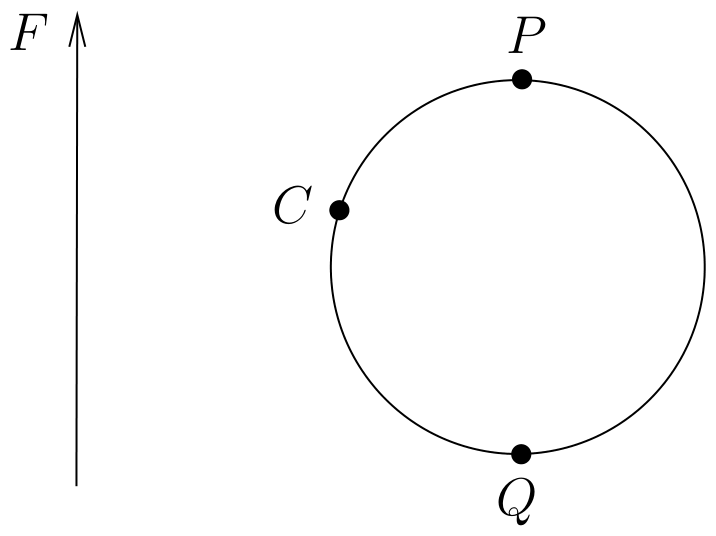
\includegraphics[width=0.42\linewidth]{fig06.png}
  \caption{带闭链 $C$ 的圆（原书 p.11）}
  \label{fig:6}
\end{figure}

此时 Morse 微分 $\mathrm{d}_{\mathrm{Morse}}=0$，但形变后的 Morse 微分 $\mathrm{d}_{\mathrm{Morse}}+m(T)$ 为
\[
  \mathrm{d}_{\mathrm{Morse}}+m(T)\colon\quad
  \begin{cases}
    [P]\mapsto (e^{T}-1)[Q],\\
    [Q]\mapsto 0.
  \end{cases}
\]
这里的形变来自
\[
  m_P^Q(T)=\#\mathcal M(P,C,Q)\,T+\#\mathcal M(P,C,C,Q)\,T^2+\cdots
  =T+\tfrac12T^2+\cdots=e^T-1.
\]
对闭链 $C$ 的每一组副本位移，从 $P$ 到 $Q$ 且按正确次序经过这些副本的梯度轨道要么恰有一条，要么一条也没有。对位移作对称化之后，就得到系数 $1/k!$。

% [Tutor Note: 为什么 $\mathrm{d}_{\mathrm{Morse}}=0$：在圆上，从极大点 $P$ 到极小点 $Q$ 恰有两条梯度轨道（沿两侧各一段半圆），二者定向相反，带符号计数相互抵消。而 $m_P^Q(T)$ 数的是经过闭链副本的轨道：对每组位移，按正确次序经过副本的轨道恰有一条，对称化后得 $1/k!$，累加即 $e^T-1=\sum_{k\ge 1}T^k/k!$。]

\textbf{通过同调扰动引理的进路。}\quad 式 (25) 可以这样证明：把 $X$ 上的微分形式复形看作双复形，第一个微分是 de Rham 微分 $\mathrm{d}_1=\mathrm{d}$，第二个微分是乘以微分形式
\[
  \mathrm{d}_2=\sum T_\alpha\,\delta^\epsilon_{C_\alpha},
\]
其中 $\delta^\epsilon_{C_\alpha}$ 是闭链的光滑化 delta 形式，见第~\ref{sec:2.3} 节。当各 $C_\alpha$ 的余维数为 1 时，这样的微分叫作 Novikov 微分 $\mathrm{d}_{\mathrm{Novikov}}=\mathrm{d}+\omega$；我们这里用的是它的显然推广。

算子 $m(T)$ 只是把第二个微分诱导到子复形（相对于 $\mathrm{d}_1$）上的结果，所用的是同调扰动引理\footnote{参看 \cite{gugenheim,lambe}。综述可参看 \cite{crainic}。拓扑量子力学的视角另见 \cite{losev}。}与 Morse 收缩。形变后的 de Rham 复形 $(\Omega^\bullet(X)[[T_\alpha]],\mathrm{d}_1+\mathrm{d}_2)$ 与形变后的 Morse 复形 $(\mathrm{MC}^\bullet(F,\mathbb R)[[T_\alpha]],\mathrm{d}_{\mathrm{Morse}}+m(T))$ 拟同构，其中 $m(T)$ 由下式给出：
\begin{equation}\tag{26}\label{eq:26}
  m(T)=p\,\mathrm{d}_2\,i^\epsilon+p\,\mathrm{d}_2K^\epsilon \mathrm{d}_2\,i^\epsilon
  +p\,\mathrm{d}_2K^\epsilon \mathrm{d}_2K^\epsilon \mathrm{d}_2\,i^\epsilon+\cdots
\end{equation}

这里 $(i^\epsilon,p,K^\epsilon)$ 是上面式 (10)、(11)、(12) 中的映射。我们假定 $\epsilon$ 足够小。事实上，把式 (26) 展开，得到
\begin{equation}\tag{27}\label{eq:27}
\begin{aligned}
  m(T)[P_i]={}&
  \lim_{\epsilon\to0}\sum_{j}\sum_{k\ge1}\sum_{\alpha_1,\dots,\alpha_k}
  \left(\int_{\mathrm{Stab}_{P_j}}\delta^\epsilon_{C_{\alpha_k}}
  K^\epsilon\bigl(\delta^\epsilon_{C_{\alpha_{k-1}}}\cdots
  \delta^\epsilon_{C_{\alpha_2}}K^\epsilon
  (\delta^\epsilon_{C_{\alpha_1}}\delta^\epsilon_{\mathrm{Unstab}_{P_i}})\cdots\bigr)
  \right)\\
  &\quad\cdot T_{\alpha_1}\cdots T_{\alpha_k}\cdot[P_j]\\
  ={}&\sum_{j}\sum_{k\ge1}\sum_{\alpha_1,\dots,\alpha_k}
  \#\mathcal M(P_i,C_{\alpha_1},\dots,C_{\alpha_k},P_j)\,
  T_{\alpha_1}\cdots T_{\alpha_k}\cdot[P_j].
\end{aligned}
\end{equation}

最后一个等号是显然的，只有序列 $C_{\alpha_1},\dots,C_{\alpha_k}$ 含重复闭链这一更微妙的情形除外。我们预期，在这种情形下，$\epsilon$-正规化给出的贡献也与注~\ref{rem:2.1} 的计数式规定一致。\footnote{例如在例~\ref{ex:4} 中，这就是一个直接的验证：取第~\ref{sec:2.3} 节意义下的正规化数据，即 $S^1\times S^1$ 上一个支撑在对角线的 $\epsilon$-邻域内的闭 1-形式 $\rho_\epsilon=f_\epsilon(\theta,\theta')\,\mathrm{d}\theta+g_\epsilon(\theta,\theta')\,\mathrm{d}\theta'$，并满足 $\int f_\epsilon\,\mathrm{d}\theta=1$、$\int g_\epsilon\,\mathrm{d}\theta'=-1$（$\theta$ 是 $S^1$ 上的角坐标）。对 $k=1,2,\dots$ 作归纳可证 $(\delta^\epsilon_C K^\epsilon)^{k-1}(\delta^\epsilon_C\delta^\epsilon_{\mathrm{Unstab}P})=\frac{1}{k!}\,\mathrm{d}\theta\,\frac{\mathrm{d}}{\mathrm{d}\theta}\bigl(\int^\theta \mathrm{d}\theta'\,f_\epsilon(\theta',\theta_0)\bigr)^k$，其中 $\theta_0$ 是 0-闭链 $C$ 的位置。由此可得 $\int_{\mathrm{Stab}Q}(\delta^\epsilon_C K^\epsilon)^{k-1}(\delta^\epsilon_C\delta^\epsilon_{\mathrm{Unstab}P})=1/k!$。}因此，带上这一保留条件，式 (26) 与计数式定义 (24) 一致。$\mathrm{d}_{\mathrm{Morse}}+m(T)$ 的平方为零这一事实，于是就是同调扰动引理的直接推论。

% [Tutor Note: 作者说“显然”，实际用到两步：其一，$\epsilon\to0$ 时 $\delta^\epsilon_C$ 弱收敛到 $\delta_C$，$K^\epsilon$ 的积分核收敛到 $\delta_{\widetilde Y}$（式 (17) 与第 2.3 节的正则化构造）；其二，沿 $X^V$ 的积分在横截性下化为交点计数。标准出处是 Gugenheim \cite{gugenheim} 与 Lambe--Stasheff \cite{lambe} 的扰动引理，综述见 Crainic \cite{crainic}。]

% ===== 第 2.5 节（原书 p.12–14） =====
\subsection{Morse 树模空间的相交公式与横截性假设}\label{sec:2.5}

\begin{takeaway}
\begin{itemize}
  \item \textbf{物理图像}：复合映射的模空间可以写成 $X^m$ 中若干拉回链的相交——每条内部边对应 $\widetilde Y_e$，每个 2 价顶点对应一条链 $Z_q$，叶子与根分别对应不稳定流形与稳定流形。
  \item \textbf{数学工具}：投影 $\pi_q,\pi_e,\pi_{\text{leaf}\,i},\pi_{\text{root}}$、链的横截相交、维数公式。
  \item \textbf{主要结论}：相交公式 (28)；横截性假设~\ref{ass:2.2} 成立时 $\mathcal M$ 是光滑整链，维数由式 (28) 后的公式给出；假设失效时模空间维数跳变（例~\ref{ex:5}）。
\end{itemize}
\end{takeaway}

考虑复合映射 (4) 的定义中出现的 Morse 树的模空间 $\mathcal M$。存在一个自然的单射，把该模空间映入 $X^m$：记录 Morse 树的三价顶点在 $X$ 中的位置，以及梯度轨道与链 $Z_{\alpha,a}$ 的交点在 $X$ 中的位置。这里 $m=r-2+\sum_i k_i$ 是相应树中内部顶点（2 价与 3 价）的总数。这一单射的像——因而 $\mathcal M$ 的一个模型——可以用 $X^m$ 中链的相交来描述：
\begin{equation}\tag{28}\label{eq:28}
\begin{aligned}
  &\mathcal M\bigl(\{Z_{\alpha,a_1}\}_{\alpha=1}^{k_1};P_{a_1a_2};
  \{Z_{\alpha,a_2}\}_{\alpha=1}^{k_2};P_{a_2a_3};\cdots;
  P_{a_{r-1}a_r};\{Z_{\alpha,a_r}\}_{\alpha=1}^{k_r};P_{a_1a_r}\bigr)\simeq{}\\
  &\qquad\sum_{\text{trees }T}
  \Biggl(\biggl(\bigcap_{e\in E}\pi_e^{-1}\widetilde Y_e\biggr)
  \cap\biggl(\bigcap_{q\in V_2}\pi_q^{-1}(Z_q)\biggr)
  \cap\biggl(\bigcap_{i=1}^{r-1}\pi_{\mathrm{leaf}\,i}^{-1}
  \bigl(\mathrm{Unstab}_{P_{a_ia_{i+1}}}\bigr)\biggr)
  \cap\pi_{\mathrm{root}}^{-1}\bigl(\mathrm{Stab}_{P_{a_1a_r}}\bigr)\Biggr).
\end{aligned}
\end{equation}

% [Tutor Note: 本段 $m=r-2+\sum_i k_i$ 中的 $m$ 是空间 $X^m$ 的指数（内部顶点总数），与复合映射 $m$ 无关；同段 $Z_{\alpha,a}$ 的下标 $a$ 与临界点 $P_{ab}$ 的双指标也各有含义，读式 (28) 时先分清这两套指标。]

其中：

\begin{itemize}
  \item 求和遍历有 $r-1$ 片叶子的有根树 $T$ 的组合类型。如上所述，边带双色 $(ab)$；沿从叶子 $(a_{i-1},a_i)$ 到叶子 $(a_i,a_{i+1})$ 的路径，会遇到 $k_i$ 个颜色为 $a_i$ 的 2 价顶点（其中叶子 $(a_r,a_1)$ 是根）。假定 $T$ 中的顶点至多为 3 价。
  \item $E$ 是内部边（不与 1 价顶点相邻的边）的集合。$V=V_2\cup V_3$ 是价不等于 1 的顶点的集合；$V_k$ 是 $k$ 价顶点的集合。
  \item 对双色为 $(a,b)$ 的边 $e$，$\widetilde Y_e$ 是与 Morse 函数 $F_a-F_b$ 相联系的 $X\times X$ 中的链 (17)。
  \item 映射 $\pi_q\colon X^V\to X$ 是到第 $q$ 个分量的投影。若 $e$ 是连接顶点 $q_1$ 与 $q_2$ 的边，则 $\pi_e\colon X^V\to X\times X$ 是选取 $X$ 的第 $q_1$ 份与第 $q_2$ 份副本的投影。$\pi_{\mathrm{leaf}\,i}\colon X^V\to X$ 选取由一条边与 $(a_i,a_{i+1})$-叶相连的顶点所对应的分量。同样，$\pi_{\mathrm{root}}\colon X^V\to X$ 选取由一条边与根相连的顶点所对应的分量。
\end{itemize}

% [Tutor Note: $\pi_e^{-1}\widetilde Y_e$ 里的波浪号不能丢：$\widetilde Y_e=\bigcup_{t>0}Y_t$ 是式 (17) 中 $X\times X$ 内的整条扩展轨道族的链，而 $Y_t$ 只是 $t$ 时刻的流动像。$\pi_e$ 把 $X^V$ 投到第 $q_1,q_2$ 份 $X\times X$，$\pi_q$ 只投到单个 $X$，两者的纤维维数不同，把 $\pi_q^{-1}(\widetilde Y_e)$ 写进公式是错的。]

关于临界点与链的序列，使复合映射 (4) 有良好定义的关键横截性假设如下。

\begin{thmenv}{假设}{2.2}\label{ass:2.2}
我们假定：式 (28) 中的输入临界点 $P_{ab}$ 与链 $Z_{\alpha,a}$ 构成的序列，满足对每棵树 $T$，式 (28) 右端的相交都是横截的。
\end{thmenv}

在此假设下，$\mathcal M$ 是 $X^m$ 中一条光滑的整链，其维数为
\[
\begin{aligned}
  \dim\mathcal M={}&\\
  ={}&(\operatorname{coind}(P_{a_1a_r})-1)
  -\sum_{i=1}^{r-1}\bigl(\operatorname{coind}(P_{a_ia_{i+1}})-1\bigr)
  -\sum_{\alpha,k}\bigl(\operatorname{codim}(Z_{\alpha,k})-1\bigr)-1.
\end{aligned}
\]

% [Tutor Note: 疑似笔误：原书 p.13 把维数公式排成两行，第一行以 $\dim\mathcal M=$ 结尾，第二行又以 $=$ 起头，于是等号出现两次。译文照印，未删去第二个等号；按上下文，第一个等号后应直接接第二行的右端。]

\begin{thmenv}{例}{5}\label{ex:5}
非横截复合的一个例子如下：$N=2$，$X$ 是作为 $\mathbb R^3$ 中单位球面实现的 2-球面，$F_1-F_2$ 取 $z$-坐标。临界点是北极 $\mathbf N$ 与南极 $\mathbf S$。设 1-闭链 $C$ 为赤道 $z=0$，$C'$ 为一个 0-闭链，即 $S^2$ 中某处的点。考虑复合 $m(\mathbf N,C,C')$：
\begin{enumerate}
  \item[(1)] 若点 $C'$ 在下半球（但不在 $\mathbf S$ 处），则存在唯一一条由 $\mathbf N$ 连到 $\mathbf S$ 且经过 $C$ 与 $C'$ 的梯度轨道，故 $m(\mathbf N,C,C')=\mathbf S$。
  \item[(2)] 若点 $C'$ 在上半球（但不在 $\mathbf N$ 处），则梯度轨道经过闭链的次序不对，故 $m(\mathbf N,C,C')=0$。
  \item[(3)] 若 $C'$ 在赤道上，横截性假设失效。
  \item[(4)] 若 $C'$ 与两个临界点 $\mathbf N$、$\mathbf S$ 之一重合，横截性假设也失效。此时从 $\mathbf N$ 到 $\mathbf S$ 且经过 $C$ 与 $C'$ 的 Morse 轨道的模空间是一维的，而预期维数为零。
\end{enumerate}
\end{thmenv}

\begin{figure}[htbp]
  \centering
  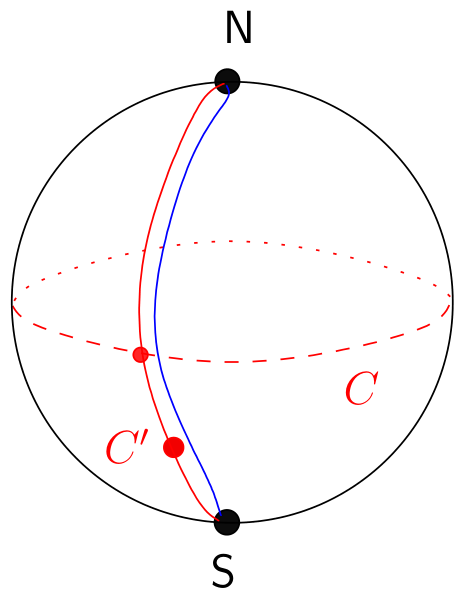
\includegraphics[width=0.30\linewidth]{fig07.png}
  \caption{经过闭链 $C$ 与 $C'$ 的梯度轨道（原书 p.13）}
  \label{fig:7}
\end{figure}

于是，横截性假设在情形 (1)、(2) 中成立，在情形 (3)、(4) 中失效。

% [Tutor Note: “预期维数为零”来自式 (28) 后的维数公式，作者没有写出代入过程：此处 $\operatorname{coind}(\mathbf S)-1=2-1=1$，$-\bigl(\operatorname{coind}(\mathbf N)-1\bigr)=-(0-1)=1$，两条链贡献 $-\bigl((1-1)+(2-1)\bigr)=-1$，最后再减 1，合计 $1+1-1-1=0$。实际模空间是一维的，故横截性必然失效。]

% ===== 第 2.6 节（原书 p.14） =====
\subsection{复合映射系数的积分公式}\label{sec:2.6}

\begin{takeaway}
\begin{itemize}
  \item \textbf{物理图像}：把相交公式里的每条链换成它的 delta 分布形式，相交数就变成 $X^V$ 上的积分；对 $\mathbb R_+^E$ 积分后，每条内部边只剩其扩展轨道族的积分核 $\delta_{\widetilde Y_e}$。
  \item \textbf{数学工具}：分布形式、积分核、波前集、横截性。
  \item \textbf{主要结论}：积分公式 (29) 与 (31)；积分号下分布形式之积有定义，由假设~\ref{ass:2.2} 保证的波前集横截性给出。
\end{itemize}
\end{takeaway}

作为式 (28) 的推论，在横截性假设下，式 (4) 中作为系数出现的 Morse 树的数目满足如下积分公式：
\begin{equation}\tag{29}\label{eq:29}
\begin{aligned}
  &\#\mathcal M\bigl(\{Z_{\alpha,a_1}\}_{\alpha=1}^{k_1};P_{a_1a_2};
  \{Z_{\alpha,a_2}\}_{\alpha=1}^{k_2};P_{a_2a_3};\cdots;
  P_{a_{r-1}a_r};\{Z_{\alpha,a_r}\}_{\alpha=1}^{k_r};P_{a_1a_r}\bigr)\\
  &\quad=\sum_{\text{trees }T}\int_{\mathbb R_+^E}\int_{X^V}
  \prod_{e\in E}\widetilde\pi_e^*\eta_e
  \prod_{q\in V_2}\pi_q^*(\delta_{Z_q})
  \prod_{i=1}^{r-1}\pi_{\mathrm{leaf}\,i}^*
  \bigl(\delta_{\mathrm{Unstab}_{P_{a_ia_{i+1}}}}\bigr)
  \cdot\pi_{\mathrm{root}}^*\bigl(\delta_{\mathrm{Stab}_{P_{a_1a_r}}}\bigr).
\end{aligned}
\end{equation}
记号与式 (28) 相同。此外：

\begin{itemize}
  \item 分布形式
  \begin{equation}\tag{30}\label{eq:30}
    \eta_e=(1-\mathrm{d}t\,\iota_v)\delta(Y_t)\in\Omega^{\dim X}(\mathbb R_+\times X\times X)
  \end{equation}
  是式 (9) 中定义的算子值微分形式 $U$ 的积分核；$U$ 与 $F_a-F_b$ 的梯度向量场相联系，其中 $(a,b)$ 是边 $e$ 的双色。
  \item 若 $e$ 是连接顶点 $q_1$ 与 $q_2$ 的边，则映射 $\widetilde\pi_e\colon\mathbb R_+^E\times X^V\to\mathbb R_+\times X\times X$ 是选取 $X$ 的第 $q_1$ 份与第 $q_2$ 份副本、以及 $\mathbb R_+$ 的第 $e$ 份副本的投影。
\end{itemize}

把 $\mathbb R_+^E$ 上的积分算出来，就可以把式 (29) 写成
\begin{equation}\tag{31}\label{eq:31}
\begin{aligned}
  \#\mathcal M={}&\sum_{\text{trees }T}\int_{X^V}
  \prod_{e\in E}\pi_e^*\delta_{\widetilde Y_e}
  \prod_{q\in V_2}\pi_q^*(\delta_{Z_q})
  \prod_{a=1}^{N-1}\pi_{\mathrm{leaf}\,a}^*
  \bigl(\delta_{\mathrm{Unstab}_{P_{a_ia_{i+1}}}}\bigr)\\
  &\quad\cdot\pi_{\mathrm{root}}^*\bigl(\delta_{\mathrm{Stab}_{P_{a_1a_r}}}\bigr).
\end{aligned}
\end{equation}
这里 $\delta_{\widetilde Y_e}$ 是非正规化 Morse 同伦 (12) 的积分核。式 (31) 积分号下各分布形式之积有良好定义，因为由假设~\ref{ass:2.2}，各波前集横截。

% [Tutor Note: 疑似笔误：式 (31) 的乘积写作 $\prod_{a=1}^{N-1}$，但被积函数里是 $\delta_{\mathrm{Unstab}_{P_{a_ia_{i+1}}}}$，下标是 $i$ 而不是 $a$；照式 (29) 应为 $\prod_{i=1}^{r-1}$，或把被积函数的下标改成 $P_{a\,a+1}$。另外这里的 $N-1$ 与式 (29) 的 $r-1$ 也不一致（$N$ 是对象个数，$r$ 是树中叶子个数）。译文照原样排印，未擅改。]

% [Tutor Note: 末句的“波前集横截”是关键：Hörmander 的波前集理论断言，两个分布之积有定义当且仅当二者的波前集沿对角逐点横截。$\delta_Z$ 的波前集是 $Z\subset X$ 的余法丛，故对 $X^V$ 上各拉回形式的乘积而言，横截性条件恰是假设~\ref{ass:2.2} 的相交横截性。可参看 Hörmander《The Analysis of Linear Partial Differential Operators》第 8 章。]

\endinput
